
%%%%%%%%%%%%%%%%%%%%%%%%%%%%%%%%%%%%%%%%%%%%%%%%%%%%%%%%
%
% Copyright (c) 2003-2010 by University of Queensland
% Earth Systems Science Computational Center (ESSCC)
% http://www.uq.edu.au/esscc
%
% Primary Business: Queensland, Australia
% Licensed under the Open Software License version 3.0
% http://www.opensource.org/licenses/osl-3.0.php
%
%%%%%%%%%%%%%%%%%%%%%%%%%%%%%%%%%%%%%%%%%%%%%%%%%%%%%%%%


\chapter{Models}
\label{MODELS CHAPTER}

The following sections give a breif overview of the model classes and their corresponding methods.

\section{The Stokes Problem}
\label{STOKES PROBLEM} 
In this section we discuss how to solve the Stokes problem which is defined as follows:

We want to calculate the velocity \index{velocity} field $v$ and pressure $p$ of an incompressible fluid \index{incompressible fluid}. They are given as the solution of the Stokes problem\index{Stokes problem}
\begin{equation}\label{Stokes 1}
-\left(\eta(v\hackscore{i,j}+ v\hackscore{j,i})\right)\hackscore{,j}+p\hackscore{,i}=f\hackscore{i}-\sigma\hackscore{ij,j}
\end{equation}
where  $f\hackscore{i}$ defines an internal force \index{force, internal} and $\sigma\hackscore{ij}$ is an initial stress \index{stress, initial}. The viscosity $\eta$ may weakly depend on pressure and velocity. If relevant we will use the notation $\eta(v,p)$ to express this dependency.

We assume an incompressible media:
\begin{equation}\label{Stokes 2}
-v\hackscore{i,i}=0
\end{equation}
Natural boundary conditions are taken in the form 
\begin{equation}\label{Stokes Boundary}
\left(\eta(v\hackscore{i,j}+ v\hackscore{j,i})\right)n\hackscore{j}-n\hackscore{i}p=s\hackscore{i} - \alpha \cdot n\hackscore{i} n\hackscore{j} v\hackscore{j}+\sigma\hackscore{ij} n\hackscore{j}
\end{equation}
which can be overwritten by constraints of the form 
\begin{equation}\label{Stokes Boundary0}
v\hackscore{i}(x)=v^D\hackscore{i}(x)
\end{equation}
at some locations $x$ at the boundary of the domain. $s\hackscore{i}$ defines a normal stress and 
$\alpha\ge 0$ the spring constant for restoring normal force.
The index $i$ may depend on the location $x$ on the boundary.
$v^D$ is a given function on the domain.

\subsection{Solution Method \label{STOKES SOLVE}}
If we assume that $\eta$ is independent from the velocity and pressure equations~\ref{Stokes 1} and~\ref{Stokes 2} 
can be written in the block form
\begin{equation}
\left[ \begin{array}{cc}
A     & B^{*} \\
B & 0 \\
\end{array} \right]
\left[ \begin{array}{c}
v \\
p \\
\end{array} \right]
=\left[ \begin{array}{c}
G \\
0 \\
\end{array} \right]
\label{STOKES}
\end{equation}
where $A$ is coercive, self-adjoint linear operator in a suitable Hilbert space, $B$ is the $(-1) \cdot$ divergence operator and $B^{*}$ is it adjoint operator (=gradient operator).
For more details on the mathematics see references \cite{AAMIRBERKYAN2008,MBENZI2005}. 

If $v\hackscore{0}$ and $p\hackscore{0}$ are given initial guesses for
velocity and pressure we calculate a correction $dv$ for the velocity by solving the first
equation of equation~\ref{STOKES}
 \begin{equation}\label{STOKES ITER STEP 1}
 A dv\hackscore{1} = G - A v\hackscore{0} - B^{*} p\hackscore{0}
\end{equation}
We then insert the new approximation $v\hackscore{1}=v\hackscore{0}+dv\hackscore{1}$ to calculate a correction $dp\hackscore{2}$
for the pressure and an additional correction $dv\hackscore{2}$ for the velocity by solving
 \begin{equation}
 \begin{array}{rcl}
 B A^{-1} B^{*} dp\hackscore{2} & = & Bv\hackscore{1} \\
 A dv\hackscore{2} & = & B^{*} dp\hackscore{2} 
\end{array}
 \label{STOKES ITER STEP 2}
 \end{equation}
The new velocity and pressure are then given by $v\hackscore{2}=v\hackscore{1}-dv\hackscore{2}$ and
$p\hackscore{2}=p\hackscore{0}+dp\hackscore{2}$ which will fulfill the block system~\ref{STOKES}. 
This solution strategy is called the Uzawa scheme \index{Uzawa scheme}. 

There is a problem with this scheme: In practice we will use an iterative scheme
to solve any problem for operator $A$. So we will be unable to calculate the operator
$ B A^{-1} B^{*}$ required for $dp\hackscore{2}$ explicitly. In fact, we need to use another
iterative scheme to solve the first equation in~\ref{STOKES ITER STEP 2} where in each iteration step
an iterative solver for $A$ is applied. Another issue is the fact that the
viscosity $\eta$ may depend on velocity or pressure and so we need to iterate over the 
three equations~\ref{STOKES ITER STEP 1} and~\ref{STOKES ITER STEP 2}. 

In the following we will use the two norms
\begin{equation}
\|v\|\hackscore{1}^2 = \int\hackscore{\Omega} v\hackscore{j,k}v\hackscore{j,k} \; dx 
\mbox{ and }
\|p\|\hackscore{0}^2= \int\hackscore{\Omega} p^2 \; dx.
\label{STOKES STOP}
\end{equation}
for velocity $v$ and pressure $p$. The iteration is terminated if the stopping criteria
 \begin{equation} \label{STOKES STOPPING CRITERIA}
\max(\|Bv\hackscore{1}\|\hackscore{0},\|v\hackscore{2}-v\hackscore{0}\|\hackscore{1}) \le \tau \cdot \|v\hackscore{2}\|\hackscore{1} 
 \end{equation}
 for a given  given tolerance $0<\tau<1$ is meet. Notice that because of the first equation of~\ref{STOKES ITER STEP 2} we have that
$\|Bv\hackscore{1}\|\hackscore{0}$ equals the
norm of $B A^{-1} B^{*} dp\hackscore{2}$ and consequently provides a norm for the pressure correction.

We want to optimize the tolerance choice for solving~\ref{STOKES ITER STEP 1}
and~\ref{STOKES ITER STEP 2}. To do this we write the iteration scheme as a fixed point problem. Here
we consider the errors produced by the iterative solvers being used. 
From Equation~\ref{STOKES ITER STEP 1} we have 
\begin{equation} \label{STOKES total V1}
v\hackscore{1} = e\hackscore{1} + v\hackscore{0} + A^{-1} ( G - Av\hackscore{0} - B^{*} p\hackscore{0} ) 
\end{equation}
where $ e\hackscore{1}$ is the error when solving~\ref{STOKES ITER STEP 1}.  
We will use a sparse matrix solver so we have not full control on the norm $\|.\|\hackscore{s}$ used in the stopping criteria for this equation. In fact we will have a stopping criteria of the form 
\begin{equation} 
\| A e\hackscore{1} \|\hackscore{s}  = \| G - A v\hackscore{1} - B^{*} p\hackscore{0} \|\hackscore{s} \le \tau\hackscore{1} \| G - A v\hackscore{0} - B^{*} p\hackscore{0} \|\hackscore{s} 
\end{equation}
where $\tau\hackscore{1}$ is the tolerance which we need to choose. This translates into the condition
\begin{equation} 
\| e\hackscore{1} \|\hackscore{1} \le K \tau\hackscore{1} \| dv\hackscore{1} - e\hackscore{1} \|\hackscore{1} 
\end{equation}
The constant $K$ represents some uncertainty combining a variety of unknown factors such as the 
norm being used and the condition number of the stiffness matrix.  
From the first equation of~\ref{STOKES ITER STEP 2} we have
\begin{equation}\label{STOKES total P2}
p\hackscore{2} =  p\hackscore{0} + (B A^{-1} B^{*})^{-1} (e\hackscore{2} + Bv\hackscore{1} )
\end{equation}
where $e\hackscore{2}$ represents the error when solving~\ref{STOKES ITER STEP 2}.
We use an iterative preconditioned conjugate gradient method (PCG) \index{linear solver!PCG}\index{PCG} with iteration 
operator $B A^{-1} B^{*}$ using the $\|.\|\hackscore{0}$ norm. As suitable preconditioner \index{preconditioner} for the iteration
operator we use $\frac{1}{\eta}$ \cite{ELMAN}, ie 
the evaluation of the preconditioner $P$ for a given pressure increment $q$ is the solution of
\begin{equation} \label{STOKES P PREC}
\frac{1}{\eta} (Pq) = q \; . 
\end{equation}
Note that in each evaluation of the iteration operator $q=B A^{-1} B^{*} s$ one needs to solve
the problem
\begin{equation} \label{STOKES P OPERATOR}
A w = B^{*} s 
\end{equation}
with sufficient accuracy to return $q=Bw$. We assume that the desired tolerance is 
sufficiently small, for instance one can take $\tau\hackscore{2}^2$ 
where $\tau\hackscore{2}$ is the tolerance for~\ref{STOKES ITER STEP 2}.

In an implementation we use the fact that the residual $r$ is given as
\begin{equation} \label{STOKES RES }
 r= B (v\hackscore{1} -  A^{-1} B^{*} dp) =  B (v\hackscore{1} - A^{-1} B^{*} dp) = B (v\hackscore{1}-dv\hackscore{2}) = B v\hackscore{2}
\end{equation}
In particular we have $e\hackscore{2} = B v\hackscore{2}$
So the residual $r$ is represented by the updated velocity $v\hackscore{2}=v\hackscore{1}-dv\hackscore{2}$. In practice, if
one uses the velocity to represent the residual $r$ there is no need 
to recover $dv\hackscore{2}$ in~\ref{STOKES ITER STEP 2} after $dp\hackscore{2}$ has been calculated.
In PCG the iteration is terminated if
\begin{equation} \label{STOKES P OPERATOR ERROR}
\| P^{\frac{1}{2}}B v\hackscore{2} \|\hackscore{0} \le \tau\hackscore{2} \| P^{\frac{1}{2}}B v\hackscore{1} \|\hackscore{0}
\end{equation}
where $\tau\hackscore{2}$ is the given tolerance. This translates into
\begin{equation} \label{STOKES P OPERATOR ERROR 2}
\|e\hackscore{2}\|\hackscore{0} = \| B v\hackscore{2} \|\hackscore{0} \le M \tau\hackscore{2} \| B v\hackscore{1} \|\hackscore{0}
\end{equation}
where $M$ is taking care of the fact that $P^{\frac{1}{2}}$ is dropped.   

As we assume that there is no significant error from solving with the operator $A$ we have 
\begin{equation} \label{STOKES total V2}
v\hackscore{2} =  v\hackscore{1} - dv\hackscore{2} 
= v\hackscore{1}  - A^{-1} B^{*}dp 
\end{equation}
Combining the equations~\ref{STOKES total V1},~\ref{STOKES total P2} and~\ref{STOKES total V2} and
setting the errors to zero we can write the solution process as a fix point problem 
\begin{equation} 
v = \Phi(v,p) \mbox{ and } p = \Psi(u,p) 
\end{equation}
with suitable functions $\Phi(v,p)$ and $ \Psi(v,p)$ representing the iteration operator without 
errors. In fact for a linear problem,  $\Phi$ and $\Psi$ are constant. With this notation we can write
the update step in the form $p\hackscore{2}= \delta p + \Psi(v\hackscore{0},p\hackscore{0})$ and 
$v\hackscore{2}= \delta v + \Phi(v\hackscore{0},p\hackscore{0})$ where 
the total error $\delta p$ and $\delta v$ are given as
\begin{equation} 
 \begin{array}{rcl}
\delta p & = &  (B A^{-1} B^{*})^{-1} ( e\hackscore{2} + B e\hackscore{1} ) \\
\delta v & = &  e\hackscore{1} -  A^{-1} B^{*}\delta p  \;.
\end{array}\label{STOKES ERRORS}
\end{equation}
Notice that $B\delta v = - e\hackscore{2}=-Bv\hackscore{2}$. Our task is now to choose the tolerances
$\tau\hackscore{1}$ and $\tau\hackscore{2}$ such that the global errors $\delta p$ and $\delta v$
do not stop the convergence of the iteration process. 

To measure convergence we use
\begin{equation} 
\epsilon = \max(\|v\hackscore{2}-v\|\hackscore{1}, \|B A^{-1} B^{*} (p\hackscore{2}-p)\|\hackscore{0})
\end{equation}
In practice using the fact that $B A^{-1} B^{*} (p\hackscore{2}-p\hackscore{0}) = B v\hackscore{1}$
and assuming that $v\hackscore{2}$ gives a better approximation to the true $v$ than
$v\hackscore{0}$ we will use the estimate
\begin{equation} 
\epsilon = \max(\|v\hackscore{2}-v\hackscore{0}\|\hackscore{1}, \|B v\hackscore{1}\|\hackscore{0})
\end{equation}
to estimate the progress of the iteration step after the step is completed. 
Note that the estimate of $\epsilon$   
used in the stopping criteria~\ref{STOKES STOPPING CRITERIA}. If $\chi^{-}$ is the convergence rate assuming
exact calculations, i.e. $e\hackscore{1}=0$ and $e\hackscore{2}=0$, we are expecting 
to maintain $\epsilon \le \chi^{-} \cdot \epsilon^{-}$. For the 
pressure increment we get:
\begin{equation} \label{STOKES EST 1}
\begin{array}{rcl}
\|B A^{-1} B^{*} (p\hackscore{2}-p)\|\hackscore{0}
 & \le & \|B A^{-1} B^{*} (p\hackscore{2}-\delta p-p)\|\hackscore{0} +
\|B A^{-1} B^{*} \delta p\|\hackscore{0} \\
 & = & \chi^{-} \cdot \epsilon^{-} + \|e\hackscore{2} + B e\hackscore{1}\|\hackscore{0}  \\
& \approx & \chi^{-} \cdot \epsilon^{-} + \|e\hackscore{2}\|\hackscore{0} \\
& \le & \chi^{-} \cdot \epsilon^{-} + M \tau\hackscore{2} \|B v\hackscore{1}\|\hackscore{0} \\  
\end{array}
\end{equation}
So we choose the value for $\tau\hackscore{2}$ from 
\begin{equation} \label{STOKES TOL2}
 M \tau\hackscore{2} \|B v\hackscore{1}\|\hackscore{0}  \le (\chi^{-})^2 \epsilon^{-}
\end{equation}
in order to make the perturbation for the termination of the pressure iteration a second order effect. We use a
similar argument for the velocity:
\begin{equation}\label{STOKES EST 2}
\begin{array}{rcl}
\|v\hackscore{2}-v\|\hackscore{1} & \le & \|v\hackscore{2}-\delta v-v\|\hackscore{1} + \| \delta v\|\hackscore{1} \\
& \le &  \chi^{-} \cdot \epsilon^{-}  + \| e\hackscore{1} -  A^{-1} B^{*}\delta p \|\hackscore{1} \\
& \approx &  \chi^{-} \cdot \epsilon^{-}  + \| e\hackscore{1} \|\hackscore{1} \\
& \le &  \chi^{-} \cdot \epsilon^{-}  +  K \tau\hackscore{1} \| dv\hackscore{1} - e\hackscore{1} \|\hackscore{1}
\\
& \le &  ( 1  + K \tau\hackscore{1}) \chi^{-} \cdot \epsilon^{-}
\end{array}
\end{equation}
So we choose the value for $\tau\hackscore{1}$ from
\begin{equation} \label{STOKES TOL1}
K \tau\hackscore{1} \le \chi^{-}
\end{equation}
Assuming we have estimates for $M$ and $K$ (if none is available, we use the value $1$.)
we can use~\ref{STOKES TOL1} and~\ref{STOKES TOL2} to get appropriate values for the tolerances. After
the step has been completed we can calculate a new convergence rate $\chi =\frac{\epsilon}{\epsilon^{-}}$. 
For partial reasons we restrict $\chi$ to be less or equal a given maximum value $\chi\hackscore{max}\le 1$.
If we see $\chi \le \chi^{-} (1+\chi^{-})$ our choices for the tolerances was suitable. Otherwise, we need to adjust the values for $K$ and $M$. From the estimates~\ref{STOKES EST 1} and~\ref{STOKES EST 2} we establish
\begin{equation}\label{STOKES EST 3}
\chi \le ( 1 + \max(M \frac{\tau\hackscore{2} \|B v\hackscore{1}\|\hackscore{0}}{\chi^{-} \epsilon^{-}},K \tau\hackscore{1}  ) ) \cdot \chi^{-} 
\end{equation}
If we assume that this inequality would be an equation if we would have chosen the right values
$M^{+}$ and $K^{+}$ then we get 
\begin{equation}\label{STOKES EST 3b}
\chi =  ( 1 + \max(M^{+} \frac{\chi^{-}}{M},K^{+} \frac{\chi^{-}}{K}) ) \cdot \chi^{-} 
\end{equation}
From this equation we set for 
than our choice for $K$ was not good enough. In this case we can calculate a new value
 \begin{equation}
K^{+} =  \frac{\chi-\chi^{-}}{(\chi^{-})^2} K
\end{equation}
In practice we will use 
 \begin{equation}
K^{+}  = \max(\frac{\chi-\chi^{-}}{(\chi^{-})^2} K,\frac{1}{2}K,1)
\end{equation}
where the second term is used to reduce a potential overestimate of $K$.  
The same identity is used for to update $M$. The updated $M^{+}$ and $K^{+}$ 
are then use in the next iteration step to control the tolerances. 

In some cases one can observe that there is a significant change 
in the velocity but the new velocity $v\hackscore{1}$ has still a 
small divergence, i.e. we have
$\|Bv\hackscore{1}\|\hackscore{0} \ll \|v\hackscore{1}-v\hackscore{0}\|\hackscore{1}$. 
In this case we will get a small pressure increment and consequently only very small changes to
the velocity as a result of the second update step which therefore can be skipped and
we can directly repeat the first update step until the increment in velocity becomes
significant relative to its divergence. In practice we will ignore the second half of the iteration step
as long as 
 \begin{equation}\label{STOKES LARGE BV1}
\|Bv\hackscore{1}\|\hackscore{0} \le \theta \cdot \|v\hackscore{1}-v\hackscore{0}\| 
\end{equation}
where $0<\theta<1$ is a given factor. In this case we will also check the stopping criteria 
with $v\hackscore{1}\rightarrow v\hackscore{2}$ but we will not correct $M$ in this case.

Starting from an initial guess $v\hackscore{0}$ and $p\hackscore{0}$ for velocity and pressure
the solution procedure is implemented as follows.
\begin{enumerate}
 \item calculate viscosity $\eta(v\hackscore{0},p)\hackscore{0}$ and assemble operator $A$ from $\eta$.
 \item calculate the tolerance $\tau\hackscore{1}$ from~\ref{STOKES TOL1}.
 \item Solve~\ref{STOKES ITER STEP 1} for $dv\hackscore{1}$ with tolerance $\tau\hackscore{1}$.
 \item update $v\hackscore{1}= v\hackscore{0}+ dv\hackscore{1}$
 \item if $Bv\hackscore{1}$ is large (see~\ref{STOKES LARGE BV1}):
 \begin{enumerate}
 \item calculate the tolerance $\tau\hackscore{2}$ from~\ref{STOKES TOL2}.
 \item Solve~\ref{STOKES ITER STEP 2} for $dp\hackscore{2}$ and $v\hackscore{2}$ with tolerance $\tau\hackscore{2}$.
 \item update $p\hackscore{2}\leftarrow p\hackscore{0}+ dp\hackscore{2}$
 \end{enumerate}
 \item else:
  \begin{enumerate}
  \item update $p\hackscore{2}\leftarrow p$ and $v\hackscore{2}\leftarrow v\hackscore{1}$
   \end{enumerate}
   \item calculate convergence measure $\epsilon$ and convergence rate $\chi$
\item if stopping criteria~\ref{STOKES STOPPING CRITERIA} holds:
 \begin{enumerate}
 \item return $v\hackscore{2}$ and $p\hackscore{2}$
 \end{enumerate}
 \item else:
 \begin{enumerate}

     \item update $M$ and $K$
     \item goto step 1 with $v\hackscore{0}\leftarrow v\hackscore{2}$ and $p\hackscore{0}\leftarrow p\hackscore{2}$.
\end{enumerate}
\end{enumerate}

\subsection{Functions}

\begin{classdesc}{StokesProblemCartesian}{domain}
opens the Stokes problem\index{Stokes problem} on the \Domain domain. The domain
needs to support LBB compliant elements for the Stokes problem, see~\cite{LBB} for details~\index{LBB condition}.
For instance one can use second order polynomials for velocity and 
first order polynomials for the pressure on the same element. Alternatively, one can use 
macro elements\index{macro elements} using linear polynomial for both pressure and velocity    with a subdivided
element for the velocity. Typically, the macro element is more cost effective. The fact that pressure and velocity are represented in different way is expressed by
\begin{python}
velocity=Vector(0.0, Solution(mesh))
pressure=Scalar(0.0, ReducedSolution(mesh))
\end{python}
\end{classdesc}

\begin{methoddesc}[StokesProblemCartesian]{initialize}{\optional{f=Data(), \optional{fixed_u_mask=Data(), \optional{eta=1, \optional{surface_stress=Data(), \optional{stress=Data()}, \optional{
restoration_factor=0}}}}}}
assigns values to the model parameters. In any call all values must be set.
\var{f} defines the external force $f$, \var{eta} the viscosity $\eta$,
\var{surface_stress} the surface stress $s$ and \var{stress} the initial stress $\sigma$.
The locations and components where the velocity is fixed are set by 
the values of \var{fixed_u_mask}. \var{restoration_factor} defines the restoring force factor $\alpha$. 
The method will try to cast the given values to appropriate 
\Data class objects.
\end{methoddesc}

\begin{methoddesc}[StokesProblemCartesian]{solve}{v,p
\optional{, max_iter=100 \optional{, verbose=False \optional{, usePCG=True }}}}
solves the problem and return approximations for velocity and pressure. 
The arguments \var{v} and \var{p} define initial guess.
\var{v} must have function space \var{Solution(domain)} and
\var{p} must have function space \var{ReducedSolution(domain)}.
The values of \var{v} marked
by \var{fixed_u_mask} remain unchanged. 
If \var{usePCG} is set to \True 
reconditioned conjugate gradient method (PCG) \index{preconditioned conjugate gradient method!PCG}  scheme is used. Otherwise the problem is solved generalized minimal residual method (GMRES) \index{generalized minimal residual method!GMRES}. In most cases 
the PCG scheme is more efficient.
\var{max_iter} defines the maximum number of iteration steps. 

If \var{verbose} is set to \True informations on the progress of of the solver are printed.
\end{methoddesc}


\begin{methoddesc}[StokesProblemCartesian]{setTolerance}{\optional{tolerance=1.e-4}}
sets the tolerance in an appropriate norm relative to the right hand side. The tolerance must be non-negative and less than 1.
\end{methoddesc}
\begin{methoddesc}[StokesProblemCartesian]{getTolerance}{}
returns the current relative tolerance.
\end{methoddesc}
\begin{methoddesc}[StokesProblemCartesian]{setAbsoluteTolerance}{\optional{tolerance=0.}}
sets the absolute tolerance for the error in the relevant norm. The tolerance must be non-negative. Typically the
absolute tolerance is set to 0.
\end{methoddesc}

\begin{methoddesc}[StokesProblemCartesian]{getAbsoluteTolerance}{}
returns the current absolute tolerance.
\end{methoddesc}

\begin{methoddesc}[StokesProblemCartesian]{getSolverOptionsVelocity}{}
returns the solver options used  solve the equations~(\ref{STOKES ITER STEP 1}) and~(\ref{STOKES P OPERATOR}) for velocity.
\end{methoddesc}

\begin{methoddesc}[StokesProblemCartesian]{getSolverOptionsPressure}{}
returns the solver options used solve the preconditioner equation~(\ref{STOKES P PREC}) for pressure.
\end{methoddesc}

\begin{methoddesc}[StokesProblemCartesian]{getSolverOptionsDiv}{}
set the solver options for solving the equation to project the divergence of the velocity onto the function space of pressure.
\end{methoddesc}


\subsection{Example: Lit Driven Cavity}
 The following script \file{lit\hackscore driven\hackscore cavity.py} 
\index{scripts!\file{helmholtz.py}} which is available in the \ExampleDirectory
illustrates the usage of the \class{StokesProblemCartesian} class to solve
the lit driven cavity problem:
\begin{python}
from esys.escript import *
from esys.finley import Rectangle
from esys.escript.models import StokesProblemCartesian
NE=25
dom = Rectangle(NE,NE,order=2)
x = dom.getX()
sc=StokesProblemCartesian(dom)
mask= (whereZero(x[0])*[1.,0]+whereZero(x[0]-1))*[1.,0] + \
      (whereZero(x[1])*[0.,1.]+whereZero(x[1]-1))*[1.,1]
sc.initialize(eta=.1, fixed_u_mask= mask)
v=Vector(0.,Solution(dom))
v[0]+=whereZero(x[1]-1.)
p=Scalar(0.,ReducedSolution(dom))
v,p=sc.solve(v,p, verbose=True)
saveVTK("u.xml",velocity=v,pressure=p)
\end{python}
 


\section{Darcy Flux}
We want to calculate the velocity $u$ and pressure $p$ on a domain $\Omega$ solving 
the Darcy flux problem \index{Darcy flux}\index{Darcy flow}
\begin{equation}\label{DARCY PROBLEM}
\begin{array}{rcl}
u\hackscore{i} + \kappa\hackscore{ij} p\hackscore{,j} & = & g\hackscore{i} \\
u\hackscore{k,k} & = & f
\end{array}
\end{equation} 
with the boundary conditions
\begin{equation}\label{DARCY BOUNDARY}
\begin{array}{rcl}
u\hackscore{i} \; n\hackscore{i}  = u^{N}\hackscore{i}  \; n\hackscore{i} & \mbox{ on } & \Gamma\hackscore{N} \\
p = p^{D} &  \mbox{ on } & \Gamma\hackscore{D} \\ 
\end{array}
\end{equation} 
where $\Gamma\hackscore{N}$ and $\Gamma\hackscore{D}$ are a partition of the boundary of $\Omega$ with $\Gamma\hackscore{D}$ non empty, $n\hackscore{i}$ is the outer normal field of the boundary of $\Omega$, $u^{N}\hackscore{i}$ and $p^{D}$ are given functions on $\Omega$, $g\hackscore{i}$ and $f$ are given source terms and $\kappa\hackscore{ij}$ is the given permability. We assume that $\kappa\hackscore{ij}$ is symmetric (which is not really required) and positive definite, i.e there are positive constants $\alpha\hackscore{0}$ and $\alpha\hackscore{1}$ wich are independent from the location in $\Omega$ such that
\begin{equation}
\alpha\hackscore{0} \; x\hackscore{i} x\hackscore{i} \le \kappa\hackscore{ij} x\hackscore{i} x\hackscore{j} \le \alpha\hackscore{1} \; x\hackscore{i} x\hackscore{i}
\end{equation}
for all $x\hackscore{i}$. 


\subsection{Solution Method \label{DARCY SOLVE}}
In practical applications it is an advantage to calculate the pressure $p$ as a correction of a 'static' pressure $p^{ref}$ which is the solution of
\begin{equation}
-(\kappa\hackscore{ki}\kappa\hackscore{kj} p\hackscore{,j}^{ref})\hackscore{,i} =  - (\kappa\hackscore{ki} (g\hackscore{k}- u^{N}\hackscore{k}))\hackscore{,i} 
\mbox{ with } 
p^{ref} = p^{D} \mbox{ on } \Gamma\hackscore{D}
\end{equation} 
With setting $u \leftarrow u-u^{N}$ and $p \leftarrow p-p^{ref}$ and 
\begin{equation}
\begin{array}{rcl}
g\hackscore{i} & \leftarrow & g\hackscore{i} - u^{N}\hackscore{i} -  \kappa\hackscore{ij} p^{ref}\hackscore{,j }\\
f & \leftarrow & f - u^{N}\hackscore{k,k}
\end{array}
\end{equation} 
we can assume that $u^{N}\hackscore{i}  \; n\hackscore{i}=0$ and 
$p^{D}=0$. 
We set 
\begin{equation}
V = \{ q \in H^{1}(\Omega) : q=0 \mbox{ on } \Gamma\hackscore{D} \}
\end{equation}
and 
\begin{equation}
W = \{ v \in (L^2(\Omega))^{d} : v\hackscore{k,k} \in L^2(\Omega) \mbox{ and } u\hackscore{i} \; n\hackscore{i} =0  \mbox{ on } \Gamma\hackscore{N} \}
\end{equation}
and define the operator $Q: V \rightarrow (L^2(\Omega))^{d}$ defined by
\begin{equation}
(Qp)\hackscore{i} = \kappa\hackscore{ij} p\hackscore{,j}
\end{equation}
and the operator $D: W \rightarrow L^2(\Omega)$ defined by 
\begin{equation}
Dv = v\hackscore{k,k}
\end{equation}
In operator notation the Darcy problem~\ref{DARCY PROBLEM} is written in the form
\begin{equation}
\begin{array}{rcl}
u + Qp & = & g \\
Du & = & f 
\end{array}
\end{equation} 
We solve this equation by minimising the functional
\begin{equation}
J(u,p):=\|u + Qp - g\|^2\hackscore{0} + \|Du-f\|\hackscore{0}^2 
\end{equation} 
over $W \times V$ where $\|.\|\hackscore{0}$ denotes the norm in $L^2(\Omega)$. A simple calculation shows that
one has to solve
\begin{equation}
( v + Qq , u + Qp - g) + (Dv,Du-f) =0 
\end{equation} 
for all $v\in W$ and $q \in V$.which translates back into operator notation
\begin{equation}
\begin{array}{rcl}
(I+D^*D)u + Qp & = & D^*f + g \\
Q^*u  + Q^*Q p & = & Q^*g \\ 
\end{array}
\end{equation} 
where $D^*$ and $Q^*$ denote the adjoint operators. 
In~\cite{LEASTSQUARESFEM1994} it has been shown that this problem is continuous and coercive in $W \times V$ and therefore has a unique solution. Also standart FEM methods can be used for discretization. It is also possible 
to solve the problem is coupled form, however this approach leads in some cases to a very ill-conditioned stiffness matrix in particular in the case of a very small or large permability ($\alpha\hackscore{1} \ll 1$ or $\alpha\hackscore{0} \gg 1$)  

The approach we are taking is to eliminate the velocity $u$ from the problem. Assuming that $p$ is known we have
\begin{equation}\label{DARCY V FORM}
v= (I+D^*D)^{-1} (D^*f + g - Qp)
\end{equation} 
(notice that $(I+D^*D)$ is coercive in $W$) which is inserted into the second equation
\begin{equation}
Q^* (I+D^*D)^{-1} (D^*f + g - Qp) + Q^* Q p = Q^*g 
\end{equation} 
which is 
\begin{equation}
Q^* ( I - (I+D^*D)^{-1} ) Q p = Q^* (g-(I+D^*D)^{-1} (D^*f + g) ) 
\end{equation} 
We use the PCG \index{linear solver!PCG}\index{PCG} method to solve this. The residual $r$ ($\in V^*$) is given as
\begin{equation}
\begin{array}{rcl}
r & = & Q^*  \left( g -(I+D^*D)^{-1} (D^*f + g) - Qp + (I+D^*D)^{-1}Q p \right)\\
& =&  Q^* \left( g- Qp - (I+D^*D)^{-1} (D^*f + g - Qp) \right) \\
& =&  Q^* \left( g - Qp - v \right)
\end{array}
\end{equation} 
So in a partical implementation we use $\hat{r}=g-Qp-v$ to represent the residual. 
The evaluation of the iteration operator for a given $p$ is then 
returning $Qp+v$ where $v$ is the solution of 
\begin{equation}\label{UPDATE W}
(I+D^*D)v = Qp
\end{equation}
We use $(Q^*Q)^{-1}$ as a preconditioner for the iteration operator $Q^* ( I - (I+D^*D)^{-1} ) Q$. So the application of the preconditioner to $\hat{r}$ representing the residual is given by solving
implemented by solving 
\begin{equation}\label{UPDATE P}
Q^*Q q  = Q^*\hat{r}
\end{equation}
The residual norm used in the PCG is given as
\begin{equation}\label{DARCY R NORM}
\|r\|\hackscore{PCG}^2 = \int r \cdot (Q^*Q)^{-1} r \; dx =\int \hat{r} \cdot Q (Q^*Q)^{-1} Q^* \hat{r} \; dx \approx
\|\hat{r}\|\hackscore{0}^2
\end{equation}
The iteration is terminated if 
\begin{equation}\label{DARCY STOP}
\|r\|\hackscore{PCG} \le \mbox{ATOL}
\end{equation}
where we set 
\begin{equation}\label{DARCY ATOL DEF}
\mbox{ATOL} = \mbox{atol} + \mbox{rtol} \cdot \left(\frac{1}{\|v\|\hackscore{0}} + \frac{1}{\|Qp\|\hackscore{0}} \right)^{-1} 
\end{equation}
where rtol is a given relative tolerance and $\mbox{atol}$ is a given absolute tolerance (typically $=0$).  
Notice that if $Qp$ and $v$ both are zero, the pair $(0,p)$ is a solution.
The problem is that ATOL is depending on the solution $p$ (and $v$ calculated form~\ref{DARCY V FORM}). In partcice one use the initial guess for $p$ 
to get a first value for ATOL. If the stopping crierion is met in the PCG iteration, a new $v$ is calculated from the current pressure approximation and ATOL is recalculated. If \ref{DARCY STOP} is still fullfilled the calculation is terminated and $(v,p)$ is returned. Otherwise PCG is restarted with a new ATOL.

\subsection{Functions}
\begin{classdesc}{DarcyFlow}{domain \optional{, adaptSubTolerance=\True}}
opens the Darcy flux problem\index{Darcy flux} on the \Domain domain.
If \var{adaptSubTolerance} is set to \True, 
the relative tolerances for solving~(\ref{DARCY V FORM}),~(\ref{UPDATE W})
and~(\ref{UPDATE P}) are set automatically.
\end{classdesc}

\begin{methoddesc}[DarcyFlow]{setValue}{\optional{f=None, \optional{g=None, \optional{location_of_fixed_pressure=None, \optional{location_of_fixed_flux=None, 
\\\optional{permeability=None}}}}}}
assigns values to the model parameters. Values can be assigned using various calls - in particular 
in a time dependend problem only values that change over time needs to be reset. The permability can be defined as scalar (isotropic), a vector (orthotropic) or a matrix (anisotropic). 
\var{f} and \var{g} are the corresponding parameters in~\ref{DARCY PROBLEM}.
The locations and compontents where the flux is prescribed are set by positive values in
\var{location_of_fixed_flux}. 
The locations where the pressure is prescribed are set by 
by positive values of \var{location_of_fixed_pressure}. 
The values of the pressure and flux are defined by the initial guess.
Notice that at any point on the boundary of the domain the pressure or the normal component of
the flux must be defined. There must be at least one point where the pressure is prescribed. 
The method will try to cast the given values to appropriate 
\Data class objects.
\end{methoddesc}

\begin{methoddesc}[DarcyFlow]{setTolerance}{\optional{rtol=1e-4}}
sets the relative tolerance \mbox{rtol} in \ref{DARCY ATOL DEF}.
\end{methoddesc}

\begin{methoddesc}[DarcyFlow]{setAbsoluteTolerance}{\optional{atol=0.}}
sets the absolute tolerance \mbox{atol} in \ref{DARCY ATOL DEF}.
\end{methoddesc}

\begin{methoddesc}[DarcyFlow]{getSolverOptionsFlux}{}
Returns the solver options used to solve the flux problems~(\ref{DARCY V FORM}) and~(\ref{UPDATE W}). Use the returned \SolverOptions object to control the solution algorithms. If the adaption of subtolerance is choosen, the tolerance will 
be overwritten before the solver is called.
\end{methoddesc}

\begin{methoddesc}[DarcyFlow]{getSolverOptionsPressure}{}
Returns the solver options used to solve the pressure problems~(\ref{UPDATE P}). 
Use the returned \SolverOptions object to control the solution algorithms. If the adaption of subtolerance is choosen, the tolerance will 
be overwritten before the solver is called. 
\end{methoddesc}

\begin{methoddesc}[DarcyFlow]{solve}{u0,p0, \optional{max_iter=100, \optional{verbose=False}}}
solves the problem. and returns approximations for the flux $v$ and the pressure $p$. 
\var{u0} and \var{p0} define initial guess for flux and pressure. Values marked
by positive values \var{location_of_fixed_flux} and \var{location_of_fixed_pressure}, respectively, are kept unchanged. \var{max_iter} sets the maximum number of iterations steps allowed for solving the coupled problem.
\end{methoddesc}


\subsection{Example: Gravity Flow}
later

%
%%%%%%%%%%%%%%%%%%%%%%%%%%%%%%%%%%%%%%%%%%%%%%%%%%%%%%%%%%%%%%%%%%%%%%%%%%%%%%
% Copyright (c) 2003-2018 by The University of Queensland
% http://www.uq.edu.au
%
% Primary Business: Queensland, Australia
% Licensed under the Apache License, version 2.0
% http://www.apache.org/licenses/LICENSE-2.0
%
% Development until 2012 by Earth Systems Science Computational Center (ESSCC)
% Development 2012-2013 by School of Earth Sciences
% Development from 2014 by Centre for Geoscience Computing (GeoComp)
%
%%%%%%%%%%%%%%%%%%%%%%%%%%%%%%%%%%%%%%%%%%%%%%%%%%%%%%%%%%%%%%%%%%%%%%%%%%%%%%

\section{Level Set Method}

The Level Set Method is used for tracking interfaces between two different types of fluids, which may have different physical parameter values for density or viscosity. The interface is represented by a signed distance function, $\phi(x)$, where the isocontour at $\phi(x)=0$ is used to defined the interface. A point in the domain can then be determined on which side of the interface it resides, based on the local sign of $\phi(x)$; for example positive $\phi(x)$ on one side of the interface and negative $\phi(x)$ on the other. Parameters values such as density and viscosity can then be defined for the two different mediums. The Level Set Method consists of two procedures, the advection and reinitialization of the signed distance function, $\phi$. The LevelSet class can be used in conjunction with the StokesProblemCartesian class for solving computational fluid dynamics problems involving the tracking of the interface. The advantage of the Level Set Method is that it can be used to track surfaces that break apart or intersect. Also, the Level Set Method avoids the need for remeshing, which is required by the Lagrangian-Eulerian (ALE) method. 

% An example of using the Level Set Method is described in the tutorial Chapter, Section %\ref{LEVELSET CHAP}.

\subsection{Solution Method}

The displacement of the interface at the zero isocontour of $\phi(x)$ is calculated each time-step by using the velocity field. This is achieved my solving the advection equation:
%
\begin{equation}
\frac{\partial \phi}{\partial t} + \vec{v} \cdot \nabla \phi = 0,
\label{ADVECTION MODELS}
\end{equation}
%
where $\vec{v}$ is the velocity field. The advection equation is solved using a Taylor-Galerkin scheme with the presence of diffusion; by expanding $\phi$ into a Taylor series:
%
\begin{equation}
\phi^{+} \simeq \phi^{-} + dt\frac{\partial \phi^{-}}{\partial t} + \frac{dt^2}{2}\frac{\partial^{2}\phi^{-}}{\partial t^{2}},
\label{TAYLOR EXPANSION MODELS}
\end{equation}
%
then by inserting
%
\begin{equation}
\frac{\partial \phi^{-}}{\partial t} = - \vec{v} \cdot \nabla \phi^{-},
\label{INSERT ADVECTION MODELS}
\end{equation}
%
and
%
\begin{equation}
\frac{\partial^{2} \phi^{-}}{\partial t^{2}} = \frac{\partial}{\partial t}(-\vec{v} \cdot \nabla \phi^{-}) = \vec{v}\cdot \nabla (\vec{v}\cdot \nabla \phi^{-}),
\label{SECOND ORDER MODELS}
\end{equation}
%
into Equation (\ref{TAYLOR EXPANSION MODELS}), the calculation of the level set function is given by:
%
\begin{equation}
\phi^{+} = \phi^{-} - dt\vec{v}\cdot \nabla \phi^{-} + \frac{dt^2}{2}\vec{v}\cdot \nabla (\vec{v}\cdot \nabla \phi^{-}).
\label{TAYLOR GALERKIN MODELS}
\end{equation}

If $\nabla \cdot \vec{v}=0$ is assumed, then the calculation of the second order derivatives in Equation (\ref{TAYLOR GALERKIN MODELS}) can be avoided.

As the computation of the distance function progresses, it becomes distorted, and so it needs to be updated in order to stay regular \cite{SUSSMAN1994}. This process is known as the reinitialization procedure. The aim is to iteratively find a solution to the reinitialization equation:
%
\begin{equation}
\frac{\partial \psi}{\partial \tau} + sign(\phi)(1 - \nabla \psi) = 0.
\label{REINITIALISATION MODELS}
\end{equation}
%
where $\psi$ shares the same level set with $\phi$, $\tau$ is pseudo time, and $sign(\phi)$ is the smoothed sign function. This equation is solved to meet the definition of the level set function, $\lvert \nabla \psi \rvert = 1$; the normalization condition. Equation (\ref{REINITIALISATION MODELS}) can be rewritten in a similar form to the advection equation:
%
\begin{equation}
\frac{\partial \psi}{\partial \tau} + \vec{w} \cdot \nabla \psi = sign(\phi),
\label{REINITIALISATION2 MODELS}
\end{equation}
%
where
%
\begin{equation}
\vec{w} = sign(\phi)\frac{\nabla \psi}{|\nabla \psi|}.
\label{REINITIALISATION3 MODELS}
\end{equation}
%
$\vec{w}$ is the characteristic velocity pointing outward from the free surface. Equation (\ref{REINITIALISATION2 MODELS}) can be solved by a similar technique to what was used in the advection step, using the Taylor-Galerkin procedure.
When the distance function, $\phi$, is calculated, the physical parameters, density and viscosity, are updated using the sign of $\phi$. The region along the interface is assumed to be of finite thickness of $\alpha h$, where $h$ is the size of the elements in the computational mesh and $\alpha$ is a smoothing parameter. The parameters are updated by the following expression:
%
\begin{equation}
P = 
\left \{ \begin{array}{l}
P_{1} \hspace{5cm}  where \ \ \psi < - \alpha h \\
P_{2} \hspace{5cm}  where \ \ \psi > \alpha h \\
(P_{2} - P_{1}) \psi/2\alpha h + (P_{1} + P_{2})/2 \ \ \ \ \ \ where \ \ |\psi| < \alpha h.
\end{array}
\right.
\label{UPDATE PARAMETERS MODELS}
\end{equation} 
%
where the subscripts $1$ and $2$ denote the different fluids.


\subsection{Functions}

\begin{classdesc}{LevelSet}{domain, func, reinit\_max, reinit\_each, tolerance, smooth}
opens the LevelSet \index{Level Set} on the \Domain domain. \var{func} defines the initial Level Set function representing the interface between two fluids. \var{reinit\_max} sets the maximum number of iterations to satisfy the normal condition, $|\nabla \phi|=1$, during the reinitialization of the Level Set function. \var{reinit\_each} sets the frequency of reinitialization for a number of time-steps. \var{tolerance} sets the convergence tolerance to satisfy the normal condition during the reinitialization of the Level Set function. \var{smooth} sets the bandwidth of size 2$\alpha h$ along the interface to smooth the physical parameters of density and viscosity; $h$ is the size of the elements in the mesh and $\alpha$ is the smoothing parameter, usually set to 1.
\end{classdesc}

\begin{methoddesc}[LevelSet]{update\_parameter}{par1, par2}
updates the physical parameters using the sign of $\phi$. \var{par1} and \var{par2} are the physical parameter values for fluid1 and fluid2 respectively. Usually this method is called twice during each time-step to update the density and viscosity of the two fluids.
\end{methoddesc}

\begin{methoddesc}[LevelSet]{update\_phi}{vel,  dt, t\_step}
updates the Level Set function. It performs the advection and reinitialization procedures. \var{vel} is the velocity field of the fluid domain, \var{dt} is the time-step size, and \var{t\_step} is the current time-step to determine when to reinitialize.
\end{methoddesc}




\section{Isotropic Kelvin Material \label{IKM}}
As proposed by Kelvin~\cite{Muhlhaus2005} material strain $D\hackscore{ij}=\frac{1}{2}(v\hackscore{i,j}+v\hackscore{j,i})$ can be decomposed into
an elastic part $D\hackscore{ij}^{el}$ and visco-plastic part $D\hackscore{ij}^{vp}$:
\begin{equation}\label{IKM-EQU-2}
D\hackscore{ij}=D\hackscore{ij}^{el}+D\hackscore{ij}^{vp}
\end{equation}
with the elastic strain given as 
\begin{equation}\label{IKM-EQU-3}
D\hackscore{ij}^{el'}=\frac{1}{2 \mu} \dot{\sigma}\hackscore{ij}'
\end{equation}
where $\sigma'\hackscore{ij}$ is the deviatoric stress (Notice that $\sigma'\hackscore{ii}=0$).
If the material is composed by materials $q$ the visco-plastic strain can be decomposed as
\begin{equation}\label{IKM-EQU-4}
D\hackscore{ij}^{vp'}=\sum\hackscore{q} D\hackscore{ij}^{q'} 
\end{equation}
where $D\hackscore{ij}^{q}$ is the strain in material $q$ given as 
\begin{equation}\label{IKM-EQU-5}
D\hackscore{ij}^{q'}=\frac{1}{2 \eta^{q}} \sigma'\hackscore{ij} 
\end{equation}
where $\eta^{q}$ is the viscosity of material $q$. We assume the following 
betwee the the strain in material $q$ 
\begin{equation}\label{IKM-EQU-5b}
\eta^{q}=\eta^{q}\hackscore{N} \left(\frac{\tau}{\tau\hackscore{t}^q}\right)^{1-n^{q}}
\mbox{ with } \tau=\sqrt{\frac{1}{2}\sigma'\hackscore{ij} \sigma'\hackscore{ij}}
\end{equation}
for a given power law coefficients $n^{q}\ge1$ and transition stresses $\tau\hackscore{t}^q$, see~\cite{Muhlhaus2005}.
Notice that $n^{q}=1$ gives a constant viscosity.
After inserting equation~\ref{IKM-EQU-5} into equation \ref{IKM-EQU-4} one gets:
\begin{equation}\label{IKM-EQU-6}
D\hackscore{ij}'^{vp}=\frac{1}{2 \eta^{vp}} \sigma'\hackscore{ij} \mbox{ with } \frac{1}{\eta^{vp}} = \sum\hackscore{q} \frac{1}{\eta^{q}} \;.
\end{equation}
and finally with~\ref{IKM-EQU-2} 
\begin{equation}\label{IKM-EQU-2bb}
D\hackscore{ij}'=\frac{1}{2 \eta^{vp}} \sigma'\hackscore{ij}+\frac{1}{2 \mu} \dot{\sigma}\hackscore{ij}'
\end{equation}
The total stress $\tau$ needs to fullfill the yield condition \index{yield condition} 
\begin{equation}\label{IKM-EQU-8c}
\tau \le \tau\hackscore{Y} + \beta \; p
\end{equation}
with the Drucker-Prager \index{Druck-Prager} cohesion factor \index{cohesion factor} $\tau\hackscore{Y}$, Drucker-Prager friction $\beta$ and total pressure $p$.
The deviatoric stress needs to fullfill the equilibrion equation
\begin{equation}\label{IKM-EQU-1}
-\sigma'\hackscore{ij,j}+p\hackscore{,i}=F\hackscore{i}
\end{equation}
where $F\hackscore{j}$ is a given external fource. We assume an incompressible media:
\begin{equation}\label{IKM-EQU-2bbb}
-v\hackscore{i,i}=0
\end{equation}
Natural boundary conditions are taken in the form 
\begin{equation}\label{IKM-EQU-Boundary}
\sigma'\hackscore{ij}n\hackscore{j}-n\hackscore{i}p=f
\end{equation}
which can be overwritten by a constraint 
\begin{equation}\label{IKM-EQU-Boundary0}
v\hackscore{i}(x)=0
\end{equation}
where the index $i$ may depend on the location $x$ on the bondary.

\subsection{Solution Method \label{IKM-SOLVE}}
By using a first order finite difference approximation wit step size $dt>0$~\ref{IKM-EQU-3} get the form
\begin{equation}\label{IKM-EQU-3b}
\dot{\sigma}\hackscore{ij}=\frac{1}{dt } \left( \sigma\hackscore{ij} - \sigma\hackscore{ij}^{-} \right)
\end{equation}
and 
\begin{equation}\label{IKM-EQU-2b}
D\hackscore{ij}'=\left(\frac{1}{2 \eta^{vp}} + \frac{1}{2 \mu dt}\right) \sigma\hackscore{ij}'-\frac{1}{2 \mu dt } \sigma\hackscore{ij}^{-'}
\end{equation}
where $\sigma\hackscore{ij}^{-}$ is the stress at the precious time step. With 
\begin{equation}\label{IKM-EQU-2c}
\dot{\gamma} = \sqrt{ 2 \left( D\hackscore{ij}' +
\frac{1}{  2 \mu \; dt} \sigma\hackscore{ij}^{-'}\right)^2}
\end{equation} 
we have
\begin{equation}
\tau = \eta\hackscore{eff} \cdot \dot{\gamma}
\end{equation} 
where
\begin{equation}
\eta\hackscore{eff}= min( \left(\frac{1}{\mu \; dt}+\frac{1}{\eta^{vp}}\right)^{-1} 
, \eta\hackscore{max}) \mbox{ with } 
\eta\hackscore{max} = \left\{ 
\begin{array}{rcl}
\frac{\tau\hackscore{Y} + \beta \; p}{\dot{\gamma}} & & \dot{\gamma}>0 \\
&\mbox{ if } \\ 
\infty & & \mbox{otherwise}
\end{array}
\right.
\end{equation}
The upper bound $\eta\hackscore{max}$ makes sure that yield condtion~\ref{IKM-EQU-8c} holds. With this setting the eqaution \ref{IKM-EQU-2b} takes the form 
\begin{equation}\label{IKM-EQU-10}
\sigma\hackscore{ij}' =  2 \eta\hackscore{eff}  \left( D\hackscore{ij}' +
\frac{1}{  2 \mu \; dt} \sigma\hackscore{ij}^{'-}\right)  
\end{equation}
After inserting~\ref{IKM-EQU-10} into~\ref{IKM-EQU-1} we get
\begin{equation}\label{IKM-EQU-1ib}
-\left(\eta\hackscore{eff} (v\hackscore{i,j}+ v\hackscore{i,j})
\right)\hackscore{,j}+p\hackscore{,i}=F\hackscore{i}+
 \left(\frac{\eta\hackscore{eff}}{\mu dt } \sigma\hackscore{ij}^{'-} \right)\hackscore{,j}
\end{equation}
Combining this with the incomressibilty condition~\ref{IKM-EQU-2} we need to solve a
Stokes problem as discussed in section~\ref{STOKES SOLVE} in each time step.

If we set 
\begin{equation}\label{IKM-EQU-44}
\frac{1}{\eta(\tau)}= \frac{1}{\mu \; dt}+\frac{1}{\eta^{vp}}
\end{equation}
we need to solve the nonlinear problem
\begin{equation}
\eta\hackscore{eff} -  min(\eta( \dot{\gamma} \cdot \eta\hackscore{eff}) 
, \eta\hackscore{max}) =0 
\end{equation}
We use the Newton-Raphson Scheme \index{Newton-Raphson scheme} to solve this problem
\begin{equation}\label{IKM-EQU-45}
\eta\hackscore{eff}^{(n+1)} = \min(\eta\hackscore{max}, 
\eta\hackscore{eff}^{(n)} -
\frac{\eta\hackscore{eff}^{(n)} - \eta( \tau^{(n)}) }
{1-\dot{\gamma} \cdot \eta'( \tau^{(n)} )} )
=\min(\eta\hackscore{max},
\frac{\eta( \tau^{(n)}) -\tau^{(n)} \cdot  \eta'( \tau^{(n)} )  }
{1-\dot{\gamma} \cdot \eta'( \tau^{(n)} )} )
\end{equation} 
where $\eta'$ denotes the derivative of $\eta$ with respect of $\tau$
and $\tau^{(n)} =  \dot{\gamma} \cdot \eta\hackscore{eff}^{(n)}$. 

Looking at the evaluation of $\eta$ in~\ref{IKM-EQU-44} it makes sense formulate
the iteration~\ref{IKM-EQU-45} using $\Theta=\eta^{-1}$. 
In fact we have 
\begin{equation}
\eta' = - \frac{\Theta'}{\Theta^2} 
\mbox{ with } 
\Theta' = \sum\hackscore{q} \left(\frac{1}{\eta^{q}} \right)'
\label{IKM iteration 7}
\end{equation} 
As
\begin{equation}\label{IKM-EQU-47}
\left(\frac{1}{\eta^{q}} \right)'
= \frac{n^{q}-1}{\eta^{q}\hackscore{N}} \cdot \frac{\tau^{n^{q}-2}}{(\tau\hackscore{t}^q)^{n^{q}-1}}
= \frac{n^{q}-1}{\eta^{q}}\cdot\frac{1}{\tau} 
\end{equation}
we have
\begin{equation}\label{IKM-EQU-48}
\Theta' = \frac{1}{\tau} \omega \mbox{ with } \omega = \sum\hackscore{q}\frac{n^{q}-1}{\eta^{q}} 
\end{equation}
which leads to 
\begin{equation}\label{IKM-EQU-49}
\eta\hackscore{eff}^{(n+1)} = \min(\eta\hackscore{max}, 
\eta\hackscore{eff}^{(n)}
\frac{\Theta^{(n)}  + \omega^{(n)}  }
{\eta\hackscore{eff}^{(n)} \Theta^{(n)^2}+\omega^{(n)} })
\end{equation} 


\subsection{Functions}

\begin{classdesc}{IncompressibleIsotropicFlowCartesian}{
domain
\optional{, stress=0
\optional{, v=0
\optional{, p=0
\optional{, t=0
\optional{, numMaterials=1
\optional{, verbose=True
\optional{, adaptSubTolerance=True
}}}}}}}}
opens an incompressible, isotropic flow problem in Cartesian cooridninates
on the domain \var{domain}.
\var{stress},
\var{v},
\var{p}, and
\var{t} set the initial deviatoric stress, velocity, pressure and time.
\var{numMaterials} specifies the number of materials used in the power law
model. Some progress information are printed if \var{verbose} is set to
\True. If \var{adaptSubTolerance} is equal to True the tolerances for subproblems are set automatically.

The domain
needs to support LBB compliant elements for the Stokes problem, see~\cite{LBB} for detials~\index{LBB condition}.
For instance one can use second order polynomials for velocity and 
first order polynomials for the pressure on the same element. Alternativly, one can use 
macro elements\index{macro elements} using linear polynomial for both pressure and velocity bu with a subdivided
element for the velocity. Typically, the macro element is more cost effective. The fact that pressure and velocity are represented in different way is expressed by
\begin{python}
velocity=Vector(0.0, Solution(mesh))
pressure=Scalar(0.0, ReducedSolution(mesh))
\end{python}
\end{classdesc}

\begin{methoddesc}[IncompressibleIsotropicFlowCartesian]{getDomain}{}
returns the domain.
\end{methoddesc}

\begin{methoddesc}[IncompressibleIsotropicFlowCartesian]{getTime}{}
Returns current time.
\end{methoddesc}

\begin{methoddesc}[IncompressibleIsotropicFlowCartesian]{getStress}{}
Returns current stress.
\end{methoddesc}

\begin{methoddesc}[IncompressibleIsotropicFlowCartesian]{getDeviatoricStress}{}
Returns current deviatoric stress.
\end{methoddesc}

\begin{methoddesc}[IncompressibleIsotropicFlowCartesian]{getPressure}{}
Returns current pressure.
\end{methoddesc}

\begin{methoddesc}[IncompressibleIsotropicFlowCartesian]{getVelocity}{}
Returns current velocity.
\end{methoddesc}

\begin{methoddesc}[IncompressibleIsotropicFlowCartesian]{getDeviatoricStrain}{}
Returns deviatoric strain of current velocity
\end{methoddesc}

\begin{methoddesc}[IncompressibleIsotropicFlowCartesian]{getTau}{}
Returns current second invariant of deviatoric stress
\end{methoddesc}

\begin{methoddesc}[IncompressibleIsotropicFlowCartesian]{getGammaDot}{}
Returns current second invariant of deviatoric strain
\end{methoddesc}


\begin{methoddesc}[IncompressibleIsotropicFlowCartesian]{setTolerance}{tol=1.e-4}
Sets the tolerance used to terminate the iteration on a time step.
\end{methoddesc}

\begin{methoddesc}[IncompressibleIsotropicFlowCartesian]{setFlowTolerance}{tol=1.e-4}
Sets the relative tolerance for the incompressible solver, see \class{StokesProblemCartesian} for details.
\end{methoddesc}

\begin{methoddesc}[IncompressibleIsotropicFlowCartesian]{setElasticShearModulus}{mu=None}
Sets the elastic shear modulus $\mu$. If \var{mu} is set to None (default) elasticity is not applied.
\end{methoddesc}

\begin{methoddesc}[IncompressibleIsotropicFlowCartesian]{setEtaTolerance=}{rtol=1.e-8}
sets the relative tolerance for the effectice viscosity. Iteration on a time step is completed if the realtive of the effective viscosity is less than \var{rtol}.
\end{methoddesc}

\begin{methoddesc}[IncompressibleIsotropicFlowCartesian]{setDruckerPragerLaw}
{\optional{tau_Y=None, \optional{friction=None}}}
Sets the parameters $\tau\hackscore{Y}$ and $\beta$ for the Drucker-Prager model in condition~\ref{IKM-EQU-8c}. If \var{tau_Y} is set to None (default) Drucker-Prager
condition is not applied.
\end{methoddesc}

\begin{methoddesc}[IncompressibleIsotropicFlowCartesian]{setElasticShearModulus}{mu=None}
Sets the elastic shear modulus $\mu$. If \var{mu} is set to None (default) elasticity is not applied.
\end{methoddesc}


\begin{methoddesc}[IncompressibleIsotropicFlowCartesian]{setPowerLaws}{eta_N, tau_t, power}
Sets the parameters of the power-law for all materials as defined in 
equation~\ref{IKM-EQU-5b}.
\var{eta_N} is the list of viscosities $\eta^{q}\hackscore{N}$,
\var{tau_t} is the list of reference stresses  $\tau\hackscore{t}^q$,
and \var{power} is the list of  power law coefficients $n^{q}$.
\end{methoddesc}


\begin{methoddesc}[IncompressibleIsotropicFlowCartesian]{update}{dt
\optional{, iter_max=100
\optional{, inner_iter_max=20
}}}
Updates stress, velocity and pressure for time increment \var{dt}.
where \var{iter_max} is the maximum number of iteration steps on a time step to
update the effective viscosity and \var{inner_iter_max} is the maximum
number of itertion steps in the incompressible solver.
\end{methoddesc}

\subsection{Example}
later

\begin{figure}
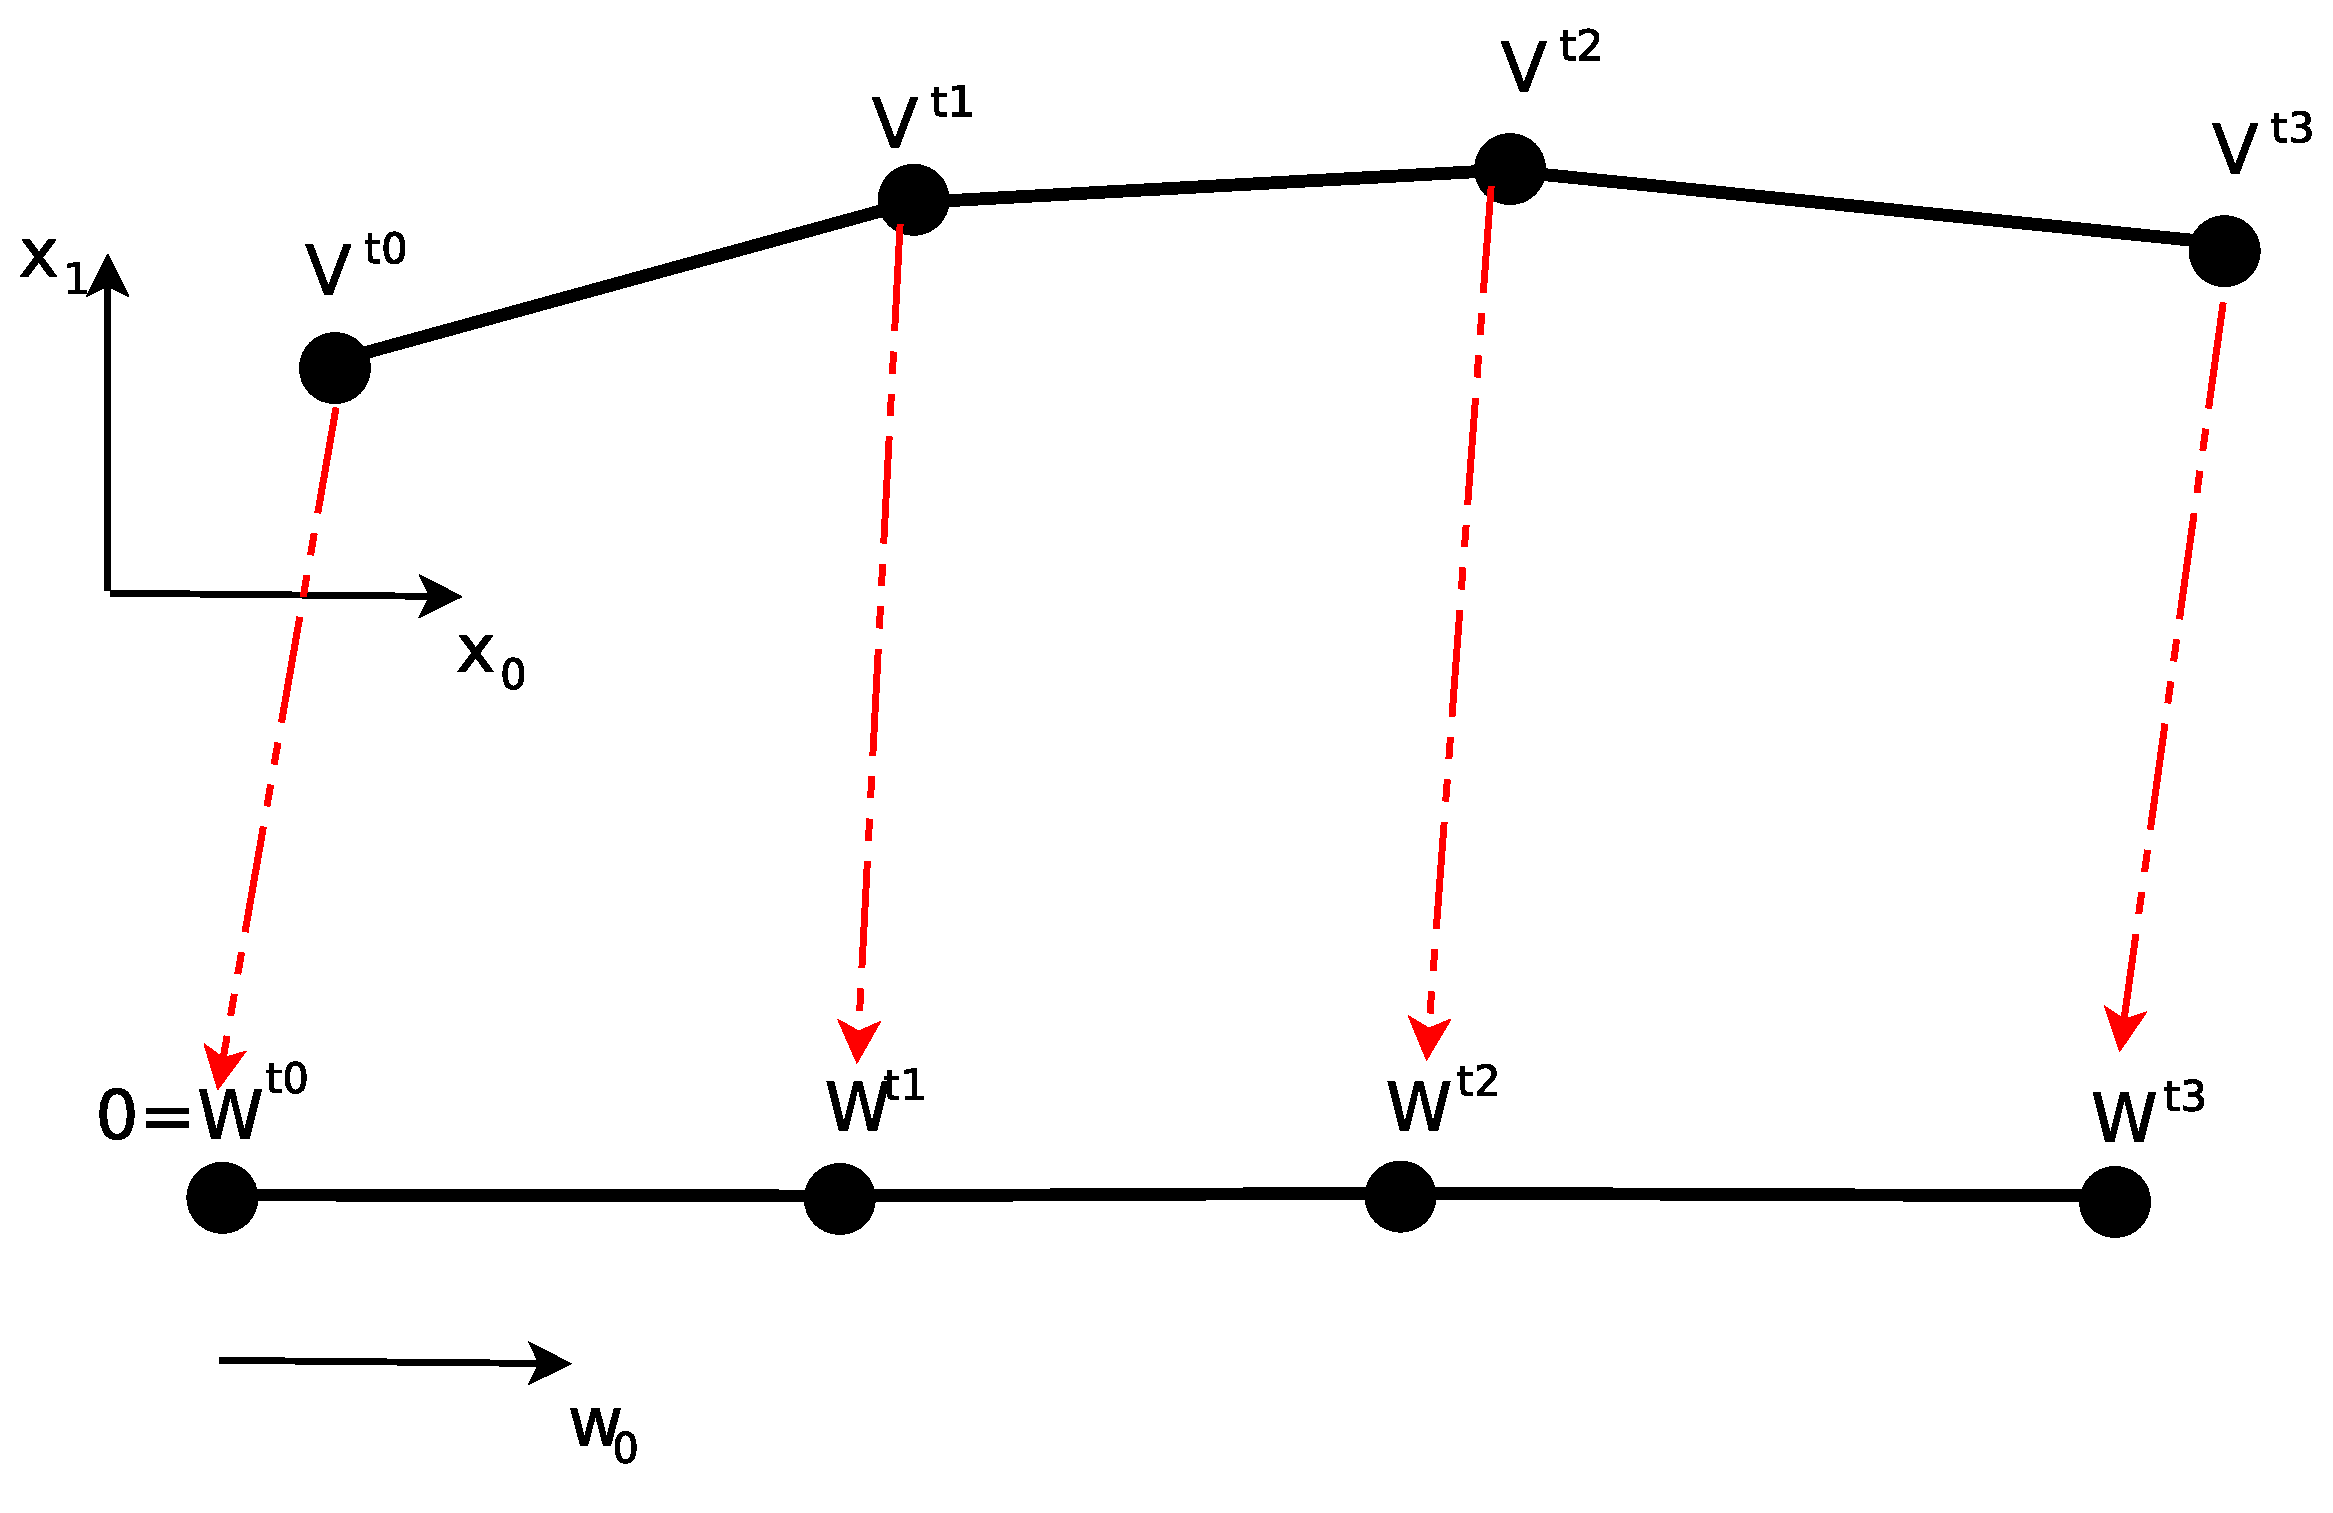
\includegraphics[width=\textwidth]{figures/FaultSystem2D}
\caption{\label{FAULTSYSTEM2D}Two dimensional fault system with one fault named `t` in the $(x\hackscore{0},x\hackscore{1})$ and its parameterization in the
$w\hackscore{0}$ space. The fault has three segments.}
\end{figure}

\section{Fault System}
\label{Fault System}
The \class{FaultSystem} is an easy to use interface to handle 2D and 3D fault systems \index{faults} as used for instance in simulating fault ruptures. The main purpose of the class is to provide a parameterization of an individual fault in the system of fault. In case of a 2D fault the fault is parameterized by a single value $w\hackscore{0}$ and in the case of a 3D fault two parameters $w\hackscore{0}$ and $w\hackscore{1}$ are used. This parameterization can be used
to impose data (e.g. a slip distribution) onto the fault. It can also be a useful tool to visualize or analyze the results on the fault if the fault is not straight. 

A fault $t$ in the fault system is represented by two polygons $(V^{ti})$ and $(v^{ti})$
defining the top and bottom line of the fault $t$.
$V^{ti}$ defines the $i$-th fault vertex at the top of the fault (typically at the surface of the Earth) and
$v^{ti}$ defines the $i$-th fault vertex at the bottom of the fault. Both polygons need to contain the same number of 
vertices. For the 2D case the polygon $(v^{ti})$ for the bottom edge of the fault is dropped. 
The patch with the vertices 
$V^{t(i-1)}$, $V^{ti}$
$v^{t(i-1)}$, and $v^{ti}$
is called the $i$-th segment of the fault `t`. In 2D the the line with the start point $V^{t(i-1)}$ 
and the end point $V^{ti}$ is called the $i$-th segment, see Figure~\ref{FAULTSYSTEM2D}.

In general a fault does not define a plane surface (or a straight line in 2D). In order to simplify working on 
a fault in a fault system a parameterization $P^t: (w\hackscore{0},w\hackscore{1}) \rightarrow (x\hackscore{0},x\hackscore{1},x\hackscore{2})$ over a rectangular domain is introduced such that 
\begin{equation}
0\le w\hackscore{0} \le w^t\hackscore{0 max} \mbox{ and }  -w^t\hackscore{1max}\le w\hackscore{1} \le 0
\label{eq:fault 1}
\end{equation}
with positive if numbers $w^t\hackscore{0 max}$ and $w^t\hackscore{1 max}$. Typically one chooses
$w^t\hackscore{0 max}$ to be the unrolled length of the fault
$w^t\hackscore{1 max}$ to be the mean value of segment depth. Moreover we have 
\begin{equation}
P^t(W^{ti})=V^{ti}\mbox{ and } P^t(w^{ti})=v^{ti}\
\label{eq:fault 2}
\end{equation}
where 
\begin{equation}
W^{ti}=(d^{ti},0) \mbox{ and } w^{ti}=(d^{ti},-w^t\hackscore{1 max})
\label{eq:fault 3}
\end{equation}
and $d^{ti}$ is the unrolled distance of $W^{ti}$ from $W^{t0}$. In the 2D case $w^t\hackscore{1 max}$ is set to zero and therefore the second component is dropped, see Figure~\ref{FAULTSYSTEM2D}.

In the case of 2D the parameterization $P^t$ is constructed as follows:
The line connecting $V^{t(i-1)}$ and $V^{ti}$ is given by
\begin{equation}
x=V^{t(i-1)} + s \cdot (V^{ti}-V^{t(i-1)})
\label{eq:2D line 1}
\end{equation}
where $s$ is between $0$ and $1$. The point $x$ is on $i$-th fault segment if and only if 
such an $s$ exists. If assume $x$ is on the fault one can calculate $s$ as
\begin{equation}
s = \frac{ (x- V^{t(i-1)})^t \cdot (V^{ti}-V^{t(i-1)}) }{\|V^{ti}-V^{t(i-1)}\|^2} 
\label{eq:2D line 1b}
\end{equation}
We then can set
\begin{equation}
w\hackscore{0}=d^{ti}+s \cdot (d^{ti}-d^{t(i-1)})
\label{eq:2D line 2}
\end{equation}
to get $P^t(w\hackscore{0})=x$.
It remains the question if the given $x$ is actual on the segment $i$ of fault $t$. To test this $s$ is restricted 
between $0$ and $1$ (so if $s<0$ $s$ is set to $0$ and if $s>1$ $s$ is set to $1$) and the we check the 
residual of equation~\ref{eq:2D line 1}, ie. $x$ is been accepted to be in the segment if
\begin{equation}
\|x-V^{t(i-1)} - s \cdot (V^{ti}-V^{t(i-1)}) \| \le tol \cdot max(\|V^{ti}-V^{t(i-1)}\|, \|x-V^{t(i-1)} \|) 
\label{eq:2D line 3}
\end{equation}
where $tol$ is a given tolerance.

ADD DISCRIPTION FOR 3D case.

\subsection{Functions}

\begin{classdesc}{FaultSystem}{
\optional{dim =3}}
Creates a fault system in the \var{dim} dimensional space.
\end{classdesc}



\begin{methoddesc}[FaultSystem]{getDim}{}
returns the spatial dimension
\end{methoddesc}
\begin{methoddesc}[FaultSystem]{getLength}{tag}
returns the unrolled length of fault \var{tag}.
\end{methoddesc}

\begin{methoddesc}[FaultSystem]{getDepth}{tag}
returns the medium depth of fault \var{tag}.
\end{methoddesc}

\begin{methoddesc}[FaultSystem]{getTags}{}
returns a list of the tags used by the fault system
\end{methoddesc}

\begin{methoddesc}[FaultSystem]{getW0Range}{tag}
returns the range of the parameterization in $w\hackscore{0}$.
For tag $t$ this is the pair $(d^{t0},d^{tn})$ where $n$ is the number of segments in the fault.
In most cases one has $(d^{t0},d^{tn})=(0,w^t\hackscore{0 max})$.
\end{methoddesc}

\begin{methoddesc}[FaultSystem]{getW1Range}{tag}
returns the range of the parameterization in  $w\hackscore{1}$.
For tag $t$ this is the pair $(-w^t\hackscore{1max},0)$.
\end{methoddesc}

\begin{methoddesc}[FaultSystem]{getW0Offsets}{tag}
returns the offsets for the parameterization of fault \var{tag}.
For tag \var{tag}=$t$ this is the list $[d^{ti}]$.
\end{methoddesc}


\begin{methoddesc}[FaultSystem]{getFaultSegments}{tag}
returns the polygons used to describe fault \var{tag}. For \var{tag}=$t$ this is the list of the vertices
$[V^{ti}]$ for the 2D and the pair of lists of the top vertices $[V^{ti}]$ and the bottom vertices  $[v^{ti}]$ in 3D.
Note that the coordinates are represented as \numpyNDA objects.
\end{methoddesc}

\begin{methoddesc}[FaultSystem]{getCenterOnSurface}{}
returns the center point of the fault system at the surfaces. In 3D the calculation of the center is
considering the top edge of the faults and projects the edge to the surface (the $x\hackscore{2}$ component is assumed to be 0). An \numpyNDA object is returned.
\end{methoddesc}

\begin{methoddesc}[FaultSystem]{getOrientationOnSurface}{}
returns the orientation of the fault system in RAD on the surface ($x\hackscore{2}=0$ plane) around the fault system center.
\end{methoddesc}
\begin{methoddesc}[FaultSystem]{transform}{\optional{rot=0, \optional{shift=numpy.zeros((3,)}}}
applies a shift \var{shift} and a consecutive rotation in the $x\hackscore{2}=0$ plane.
\var{rot} is a float number and \var{shift} an \numpyNDA object.
\end{methoddesc}

\begin{methoddesc}[FaultSystem]{addFault}{top, tag \optional{, bottom=None \optional{, w0_offsets=None\optional{, w1_max=None}}}}
adds the  fault \var{tag} to the fault system. 

\var{top} is the list of the vertices defing the top of the fault
while \var{bottom} is the list of the vertices defing the bottom of the fault.
In the case of 2D \var{bottom} must not be present. Both list, if present, must have the same length.
\var{w1_max} defines the range of the $w\hackscore{1}$. If not present the mean value over the depth of 
all segment edges in the fault is used.
\var{w0_offsets} sets the offsets $d^{ti}$. If not present it i chosen such that $d^{ti}-d^{t(i-1)}$ is the length of the $i$-th segment. In some cases, eg. when kinks in the fault are relevant, it can be useful
to explicitly specify the offsets in order to simplify the assignment of values.
\end{methoddesc}

\begin{methoddesc}[FaultSystem]{getMaxValue}{f\optional{, tol=1.e-8}}
returns the maximum value of \var{f}, the fault where the maximum is found and the location on the fault in fault coordinates. \var{f} must be a \Scalar. When the maximum is calculated only \DataSamplePoints are considered
which are on a fault in the fault system in the sense of condition~\ref{eq:2D line 3} or \ref{eq:3D line 3}, respectively. In the case no \DataSamplePoints is found the returned tag is \var{None} and
the maximum value as well as the location of the maximum value are undefined.
\end{methoddesc}

\begin{methoddesc}[FaultSystem]{getParametrization}{x,tag \optional{\optional{, tol=1.e-8}, outsider=None}}
returns the argument $w$ of the parameterization $P^t$ for \var{tag}=$t$ to provide \var{x}
together with a mask indicating where the given location if on a fault in the fault system by the value $1$ (otherwise the value is set to $0$). \var{x} needs to be \Vector or \numpyNDA object. \var{tol} defines the tolerance to decide if a given \DataSamplePoints is on fault \var{tag}. The value
\var{outside} is the value used as a replacement value for $w$ where the corresponding value in \var{x} is not 
on a fault. If not \var{outside} is not present an appropriate value is used.
\end{methoddesc}

\begin{methoddesc}[FaultSystem]{getSideAndDistance}{x,tag}
returns the side and the distance at locations \var{x} from the fault \var{tag}.
\var{x} needs to be \Vector or \numpyNDA object. Positive values for side means that the corresponding location is 
to the right of the fault, a negative value means that the corresponding location is 
to the left of the fault. The value zero means that the side is undefined.
\end{methoddesc}

\subsection{Example}
See section~\ref{Slip CHAP}









% \section{Drucker Prager Model}